% !TEX program = lualatex
\documentclass[12pt,a4paper]{article}
\usepackage{fontspec}
\setmonofont{Latin Modern Mono}
\usepackage{xcolor}
\usepackage{listings}
\usepackage{geometry}
\usepackage{fancyhdr}
\usepackage{hyperref}
\usepackage{graphicx}
\geometry{margin=1in}
\usepackage{multicol}

% -------------------------------
% SOLUTION TOGGLE
% -------------------------------
\newif\ifshowsolutions
\showsolutionstrue 
% \showsolutionsfalse

% -------------------------------
% Header and Footer Configuration
% -------------------------------
\pagestyle{fancy}
\fancyhf{}
\lhead{Lab Mid}
\rhead{CSE 4308: DBMS Lab}
\cfoot{\thepage}
\setlength{\headwidth}{\textwidth}

% -------------------------------
% Code Listing Style
% -------------------------------
\definecolor{codegreen}{rgb}{0,0.6,0}
\definecolor{codegray}{rgb}{0.5,0.5,0.5}
\definecolor{codepurple}{rgb}{0.58,0,0.82}
\definecolor{backcolour}{rgb}{0.95,0.95,0.92}

\lstdefinestyle{mystyle}{
    backgroundcolor=\color{backcolour},
    commentstyle=\color{codegreen},
    keywordstyle=\color{magenta},
    numberstyle=\tiny\color{codegray},
    stringstyle=\color{codepurple},
    basicstyle=\ttfamily\footnotesize,
    breaklines=true,
    captionpos=b,
    keepspaces=true,
    numbers = none,
    numbersep=5pt,
    tabsize=2,
    frame=single,
    columns=fullflexible,
    showspaces=false,
    showstringspaces=false,
    showtabs=false
}

\lstset{style=mystyle}

% Images: found next to this file (local compile_labs.sh) or via the
% lab folder when compiled from the project root (Overleaf).
\graphicspath{{lab_08_mid/}}

\begin{document}

% --------------------------------------------------------------
% TITLE PAGE
% --------------------------------------------------------------
\begin{titlepage}
    \centering
    \vspace*{2\baselineskip}

    \rule{14cm}{2pt}\vspace*{-0.8\baselineskip}\vspace*{1.5pt}
    \rule{14cm}{0.5pt}\vspace{2\baselineskip}

    {\Huge\bfseries\scshape Lab Mid\par}
    \vspace{3mm}
    {\Large }
    \vspace{3mm}

    \rule{14cm}{0.5pt}\vspace*{-0.7\baselineskip}\vspace{2.5pt}
    \rule{14cm}{2pt}

    \vspace{2\baselineskip}

    {\Large\bfseries CSE 4308\par}
    \vspace{1\baselineskip}
    {\large DATABASE MANAGEMENT SYSTEMS LAB\par}

    \vfill
    {\normalsize Prepared by:\\ Samnun Azfar, Jr. Lecturer, CSE\\ Samia Nawsheen, Jr. Lecturer, CSE\par}
    {\normalsize Academic Year: AY25-26\par}
\end{titlepage}

\newpage
\newpage

% ==============================================================
\section*{DBMS Lab Midterm}

\begin{figure}[h]
        \centering
        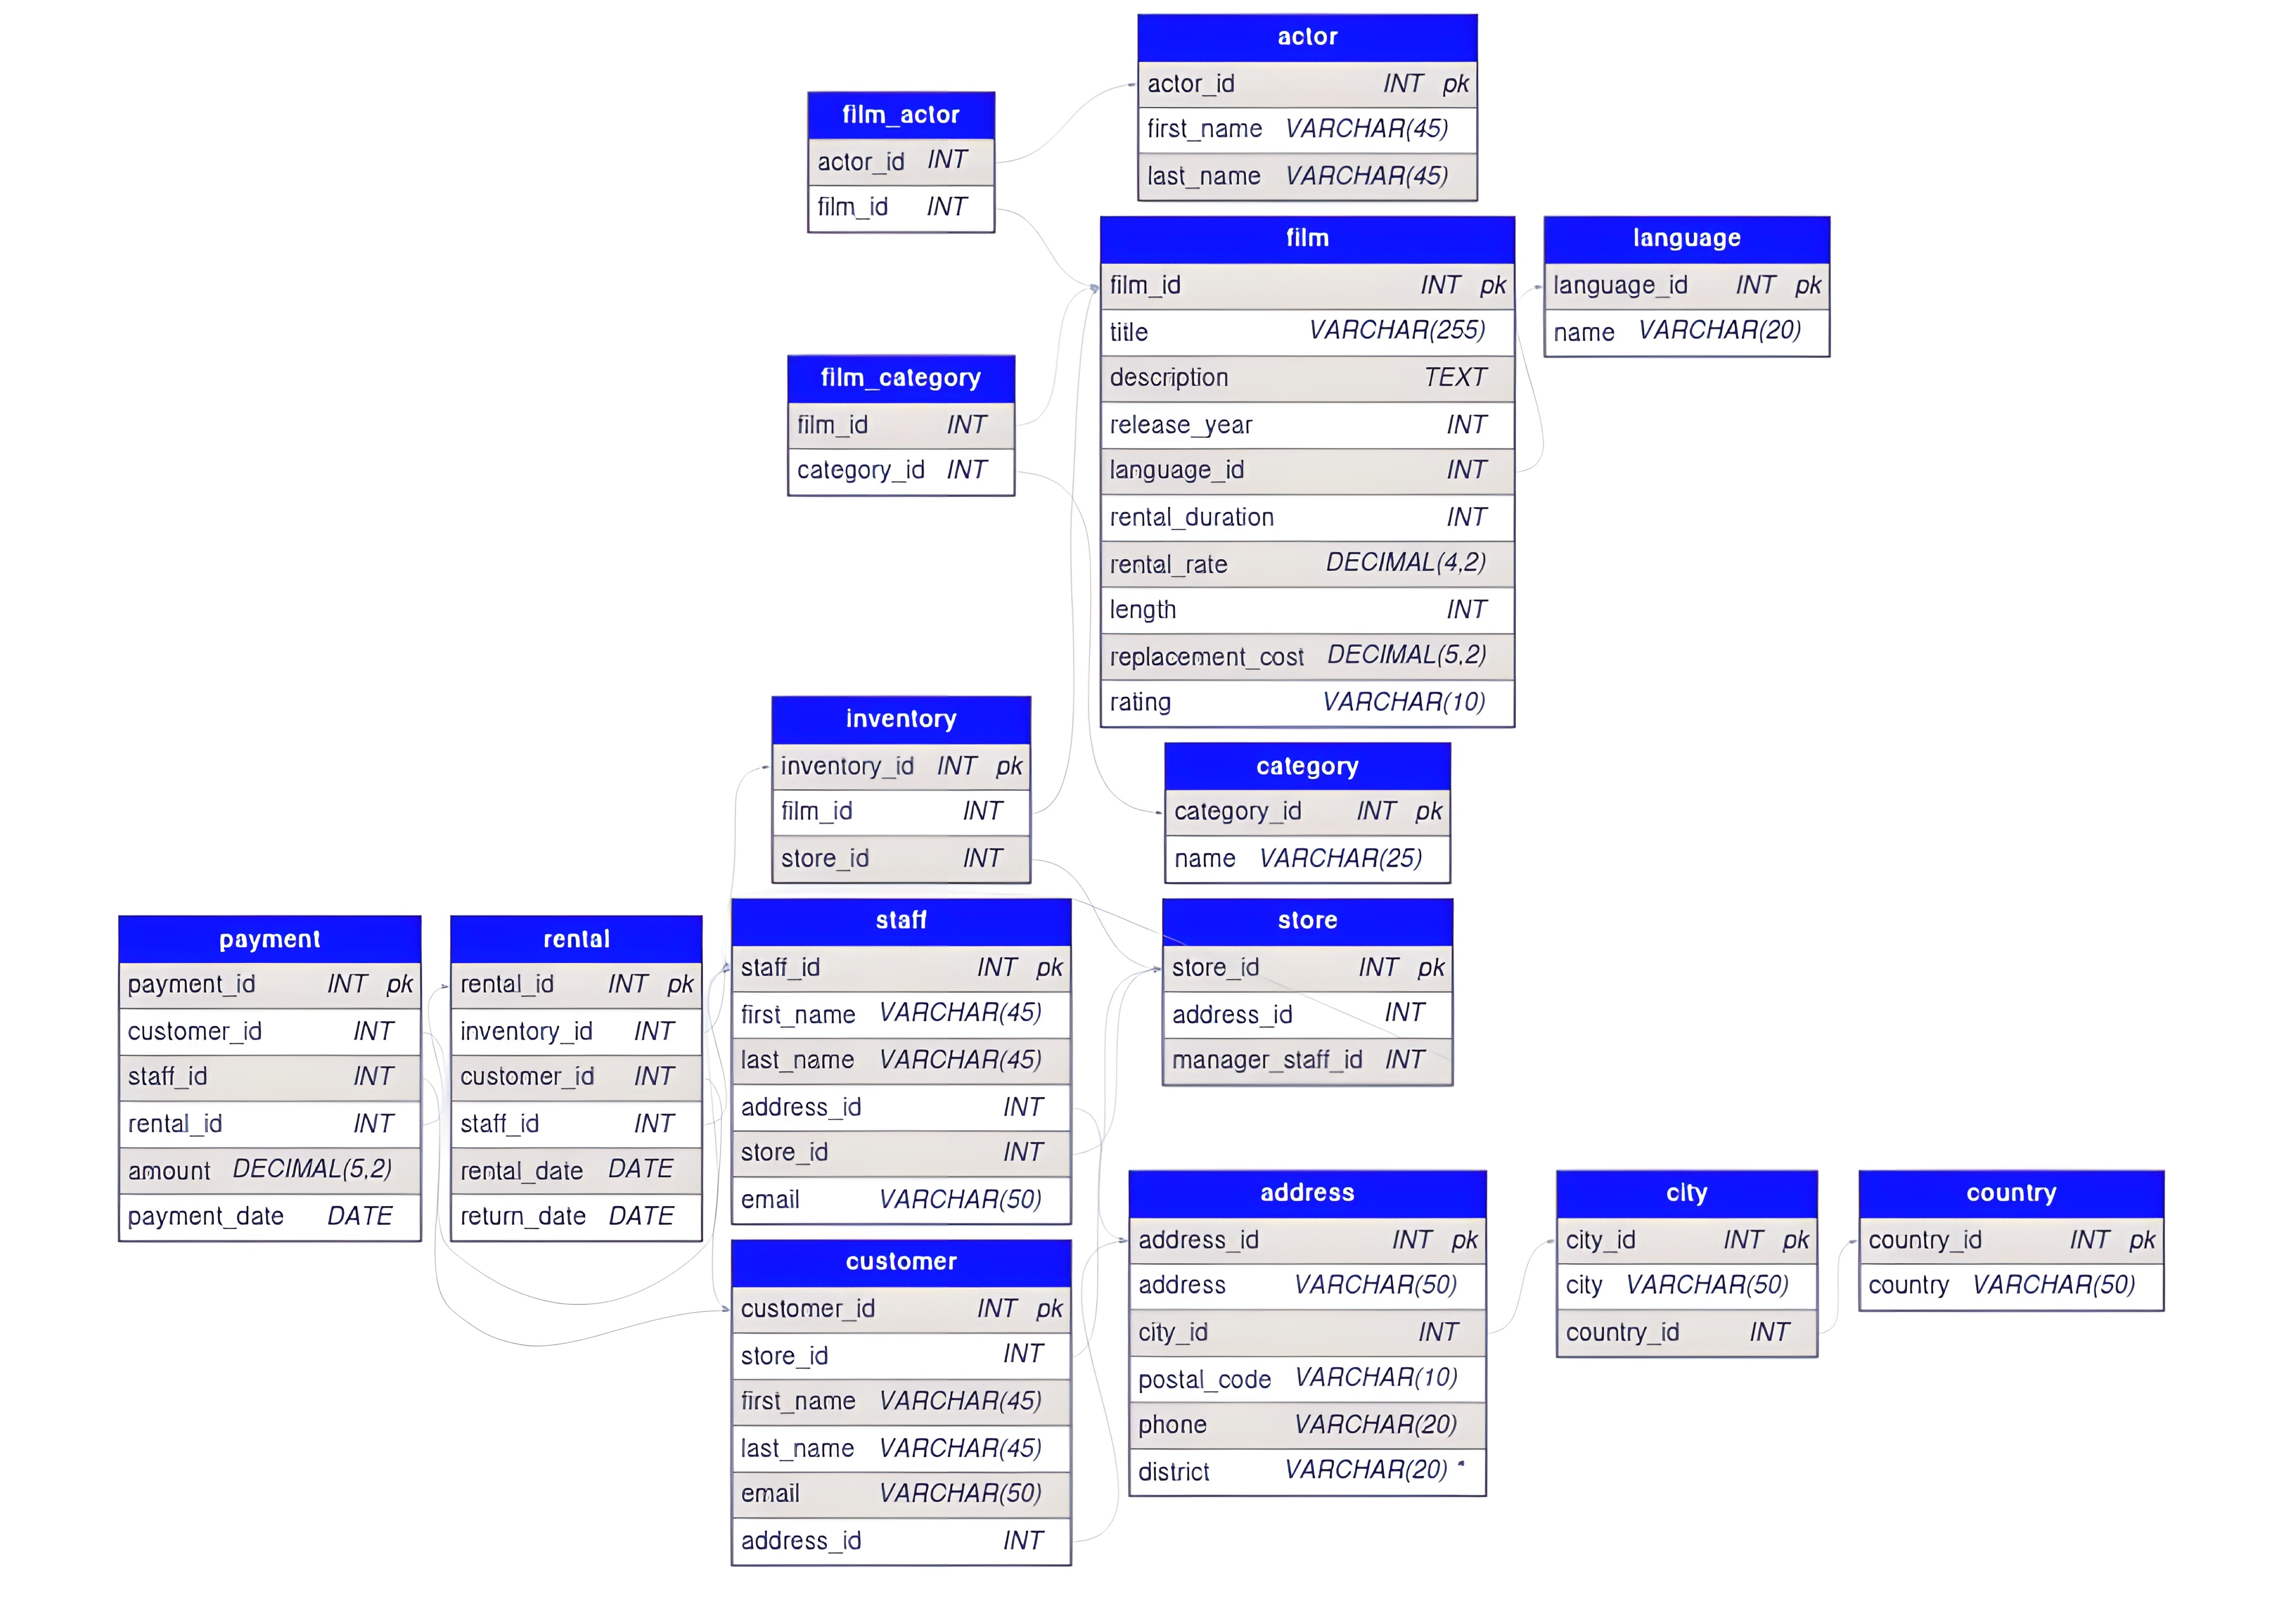
\includegraphics[width=\linewidth]{lab_08_dvdrental_1.png}
\end{figure}

\begin{enumerate}

    \item List all customers whose email contains the domain \texttt{.net}.

    \ifshowsolutions
    \begin{lstlisting}[language=SQL]
    SELECT first_name, last_name, email
    FROM customer
    WHERE email LIKE '%.net%';
    \end{lstlisting}
    \fi

    \item Find the titles of films that have ratings G or PG.

    \ifshowsolutions
    \begin{lstlisting}[language=SQL]
    SELECT title
    FROM film
    WHERE rating IN ('G', 'PG');
    \end{lstlisting}
    \fi

    \item Identify all films whose titles contain exactly two words.

    \ifshowsolutions
    \begin{lstlisting}[language=SQL]
    SELECT title
    FROM film
    WHERE LENGTH(TRIM(title)) - LENGTH(REPLACE(TRIM(title), ' ', '')) = 1;
    \end{lstlisting}
    \fi

    \item Show the number of customers who have made payments and who have never made a payment.

    \ifshowsolutions
    \begin{lstlisting}[language=SQL]
    SELECT
    (SELECT COUNT(DISTINCT customer_id) FROM payment) AS paid,
    (SELECT COUNT(*) 
     FROM customer
     WHERE customer_id NOT IN (
         SELECT customer_id FROM payment
     )) AS unpaid;
    \end{lstlisting}
    \fi

    \item Display each store ID along with the total number of customers registered in that store.

    \ifshowsolutions
    \begin{lstlisting}[language=SQL]
    SELECT store_id, COUNT(*) AS total_customers
    FROM customer
    GROUP BY store_id;
    \end{lstlisting}
    \fi

    \item Find the film categories whose average rental rate is greater than 3.

    \ifshowsolutions
    \begin{lstlisting}[language=SQL]
    SELECT c.name, AVG(f.rental_rate) AS avg_rate
    FROM category c
    JOIN film_category fc ON c.category_id = fc.category_id
    JOIN film f ON fc.film_id = f.film_id
    GROUP BY c.name
    HAVING AVG(f.rental_rate) > 3;
    \end{lstlisting}
    \fi

    \item List customers who have rented at least one film with a rental rate above 4.

    \ifshowsolutions
    \begin{lstlisting}[language=SQL]
    SELECT DISTINCT c.customer_id, c.first_name, c.last_name
    FROM customer c
    WHERE c.customer_id IN (
        SELECT r.customer_id
        FROM rental r
        JOIN inventory i ON r.inventory_id = i.inventory_id
        JOIN film f ON i.film_id = f.film_id
        WHERE f.rental_rate > 4
    );
    \end{lstlisting}
    \fi

    \item Show rentals where the return date was exactly the same as the rental date.

    \ifshowsolutions
    \begin{lstlisting}[language=SQL]
    SELECT rental_id, rental_date, return_date
    FROM rental
    WHERE EXTRACT(DAY FROM (return_date - rental_date)) = 0;
    \end{lstlisting}
    \fi

    \item Identify customers who have rented more films than the average number of rentals per customer.

    \ifshowsolutions
    \begin{lstlisting}[language=SQL]
    SELECT c.customer_id, c.first_name, c.last_name
    FROM customer c
    JOIN rental r ON c.customer_id = r.customer_id
    GROUP BY c.customer_id, c.first_name, c.last_name
    HAVING COUNT(r.rental_id) > (
        SELECT AVG(rental_count)
        FROM (
            SELECT COUNT(*) AS rental_count
            FROM rental
            GROUP BY customer_id
        ) sub
    );
    \end{lstlisting}
    \fi

    \item Find films that have been rented more times than the average number of rentals per film.

    \ifshowsolutions
    \begin{lstlisting}[language=SQL]
    SELECT f.film_id, f.title, COUNT(r.rental_id) AS rental_count
    FROM film f
    JOIN inventory i ON f.film_id = i.film_id
    JOIN rental r ON i.inventory_id = r.inventory_id
    GROUP BY f.film_id, f.title
    HAVING COUNT(r.rental_id) > (
        SELECT AVG(film_rental_count)
        FROM (
            SELECT COUNT(r2.rental_id) AS film_rental_count
            FROM inventory i2
            JOIN rental r2 ON i2.inventory_id = r2.inventory_id
            GROUP BY i2.film_id
        ) sub
    );
    \end{lstlisting}
    \fi

\end{enumerate}

\end{document}